\subsection{Notary Scheme}
\label{sec:notary}
\subsubsection{Ripple Interledger protocol}
\label{subsec:interledger}
\noindent Earlier the discussion is focused on cross-chain, this project is more focused on cross-ledger, which means that the agreement supports not only decentralized blockchains but also supports various centralized ledgers. This project provides broader support for cross-chain applications. Interledger protocol has evolves many version right now, here we introduces the version explained by white paper~\cite{thomas2015protocol}.\\

\noindent Ripple is the first project to propose the use of blockchain technology to achieve cross-ledger exchange of assets, with a focus on resolving cross-border remittances, enabling faster and more economical international remittances via the Ripple network.\\

\noindent Interledger Protocol(ILP)~\cite{thomas2015protocol} is compatible with any online ledger systems. Specifically, the ILP will establish a two-way relationship between the trader's account and a Ripple local account, enabling simultaneous changes between the two to ensure transparency in the transaction process. At the same time, for two ledger systems that do not have a direct payment channel, multi-hop indirect cross-ledger transactions can be realized through ILP. \\

\noindent The main idea of ILP is to secure cross-ledger transactions by setting up \textit{escrow account} on Ripple. So the process will need the preparation of escrow account of several parties in the transaction. As an example, in Figure \ref{fig:ILP}Bob, and one selected market maker should have their Ripple escrow accounts set up on two bank systems before the transaction. \\

\begin{itemize}
    \item Alice first selects a market maker with the most suitable exchange rate, and fill in the remittance information, receipt address and timeout period on the Ripple application.
    \item The Interledger module will pack this information and sent to the Ripple Account 1, Ripple Account 1 records the changed amount of currency in the escrow account 1 and sends the transfer certificate to the \textbf{Validator}
    \item For Bob, company B fills in the Ripple application with information such as the remittance address and timeout period and broadcasts it on the Ripple network. At this time, the liquidity provider selected by A will transfer a certain amount of assets in B's currency from Ripple $Acc.3$ to Ripple $Acc.2$ in advance, then send the transfer certificate to the \textbf{Validator}
    \item Validator checks the two transfer certificates; after the verification is passed, the ILP ledger will be liquidated simultaneously according to the Hashed Time Lock Agreement.
    \item The final step is when liquidation completed, Ripple will synchronize all account changes through an interledger module, thus realizing the cross-ledger transactions.
\end{itemize}
        \begin{figure}[H]
        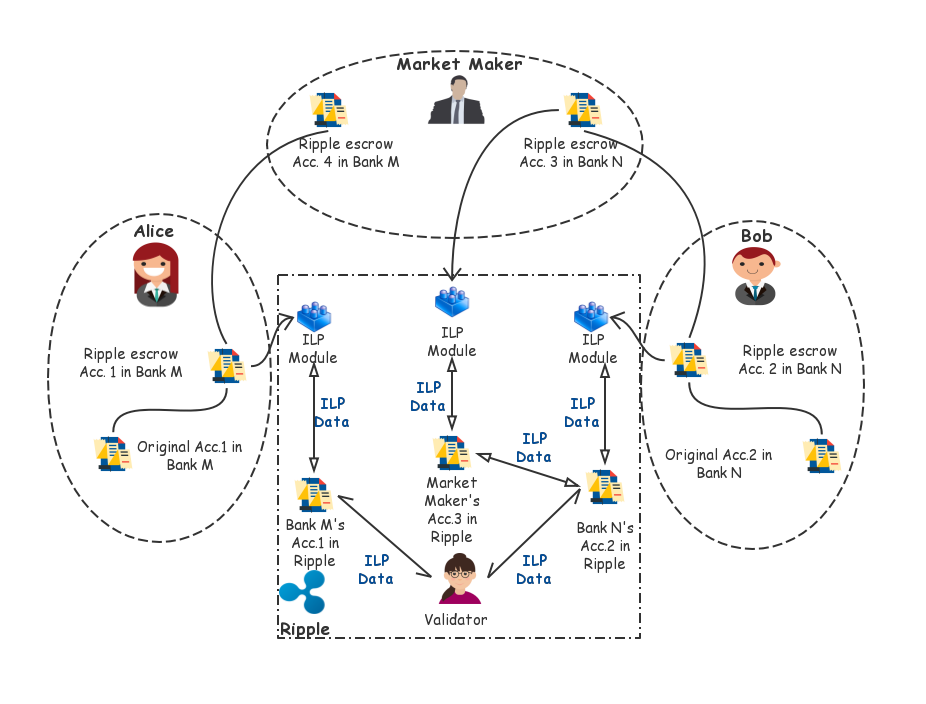
\includegraphics[width=1\textwidth]{./figures/ILP.png}
        \centering
        \caption{ILP example process}%\protect\footnotemark}
        \centering
        \label{fig:ILP}
        \end{figure}
        

\subsubsection{Wanchain}
\noindent Wanchain\cite{wanchain.org} is a cross-chain platform project initiated in 2016. It is a heterogeneous cross-chain framework that implements cross-chain communications based primarily on distributed notary scheme. This model mainly uses cryptography "Secure Multi-Party Computation" and "Threshold Key Sharing Scheme" to achieve the Authenticator distributed signature.\\

\noindent Wanchain provides the infrastructure for asset cross-chain transfer channels for different blockchain networks, realizing the transfer of assets between Wanchain and original chain. Wanchain 3.0 now launches bridges from Bitcoin to the Ethereum network. The transaction reliability verification is completed by multiple \textbf{Storeman} nodes of Wanchain. The following figures~\ref{fig:wan1} and~\ref{fig:wan2} are shown the transfer process between Wanchain and Ethereum.

        \begin{figure}[H]
        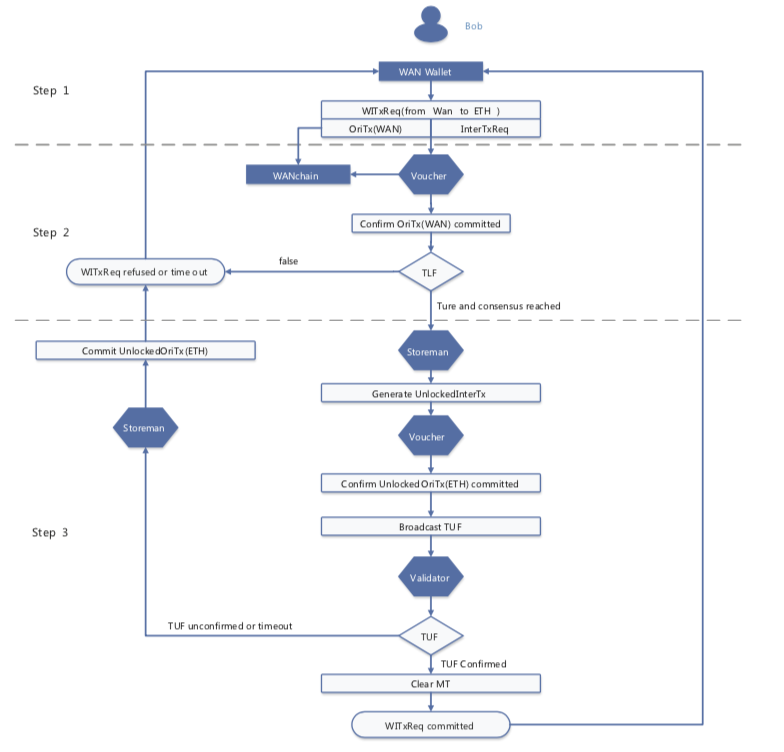
\includegraphics[width=1\textwidth]{./figures/ethtowan.png}
        \centering
        \caption{{Data transfer process from Ethereum to Wanchain}\protect\footnotemark}
        \centering
        \label{fig:wan1}
        
        \end{figure}
\footnotetext{Image courtesy of Wanchain white paper\cite{wanchain.org}}
        \begin{figure}[H]
        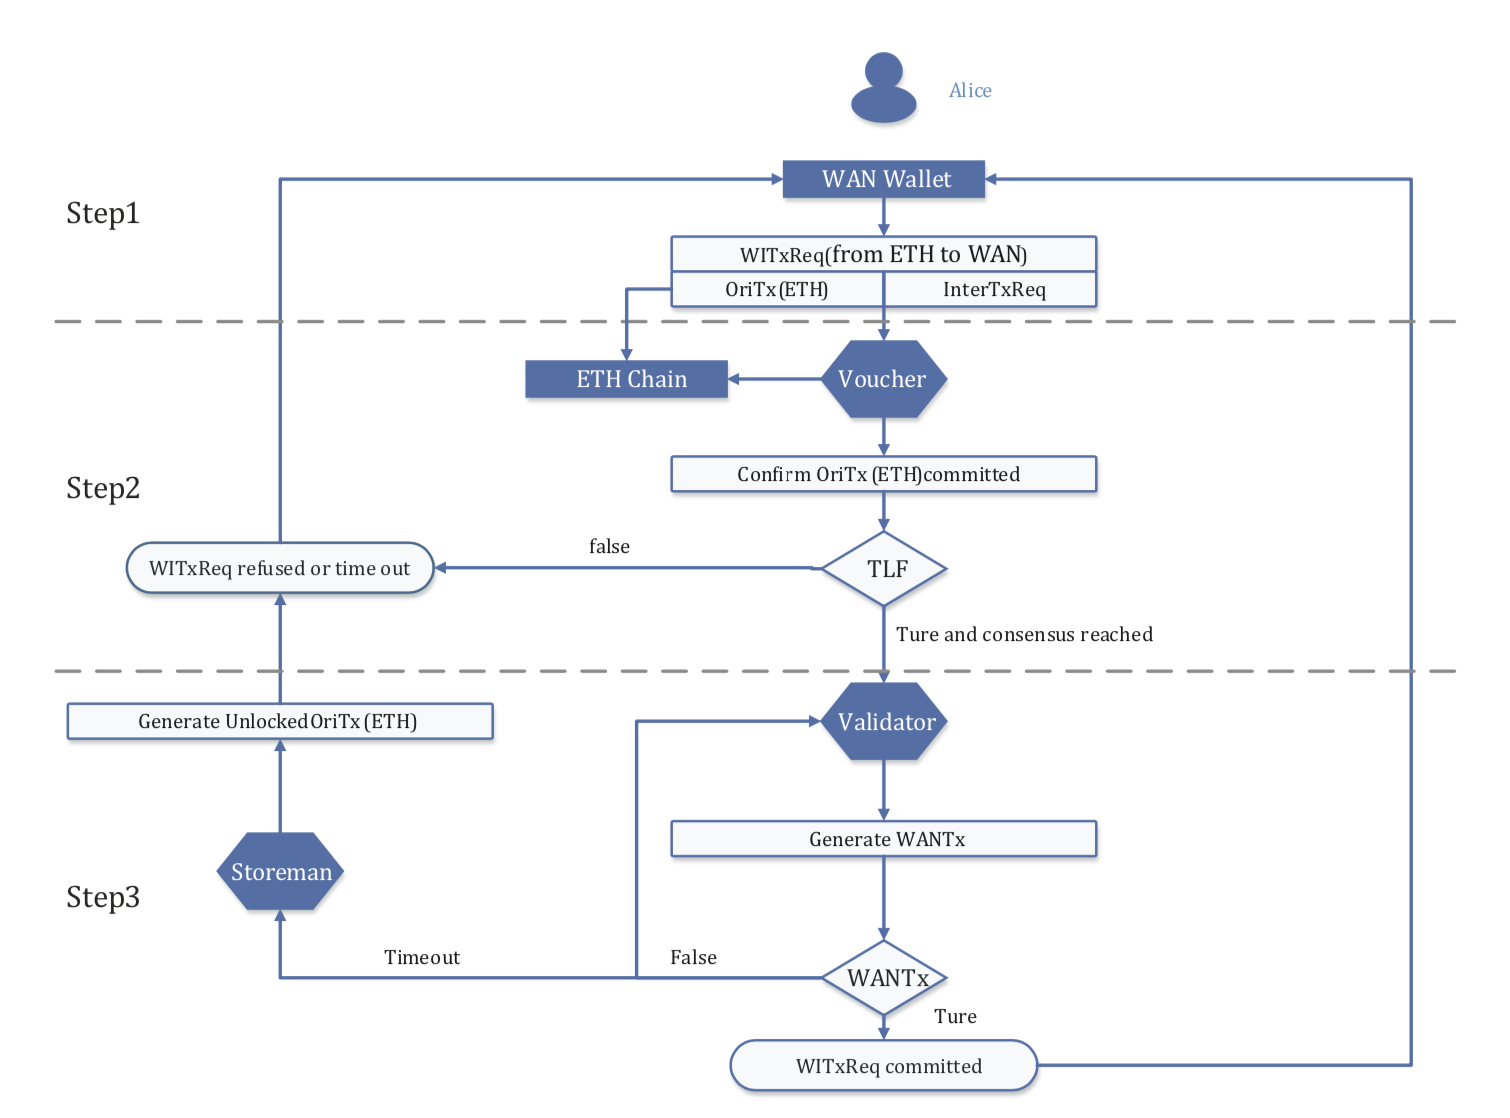
\includegraphics[width=0.88\textwidth]{./figures/wantoeth.png}
        \centering
        \caption{{Data transfer process from Wanchain to Ethereum}\protect\footnotemark}
        \centering
        \label{fig:wan2}
        
        \end{figure}
\footnotetext{Image courtesy of Wanchain white paper\cite{wanchain.org}}

\begin{itemize}

    \item The token of the user in the original chain will be sent to Wanchain in the locked account, and Hash Time Lock locks the transaction;
    \item After the \textbf{Voucher} verified  the transaction on the original chain, the \textbf{Storeman} will initiate a cross-chain contract transaction on the Wanchain, and transfer the mapping token in Wanchain to the user's exchange account on Wanchain, and locked;
    \item After the user's wallet detects the transaction locked by the cross-chain contract, it releases the secret to the cross-chain contract;
    \item Storeman obtains the control of the original chain token through the secret, thus achieving confirmation of the original chain transaction.
    \item If the user does not release the secret within the scope of the hash time lock, the hash time lock expires
    \item The transaction of the contract is automatically invalidated, and the user regains control of the original token.
\end{itemize}
\noindent In Wanchain, when Storeman locked an account, the private key of the locked account is scattered into multiple pieces and send to Storeman, and it requires more than a certain percentage of Storeman complete the signature before the final confirmation. To avoid conspiracy, Storeman has to pay a certain amount of token to participate in the verification in case of doing evil. To ensure atomicity, Wanchain uses a hash time lock to lock cross-chain transactions, ensuring that no user or Storeman will complete a one-sided transaction.\\

\noindent Since the Wanchain mechanism does not change the original chain. It is necessary to adapt the development according to the characteristics of the original chain, which is also the difficulty of heterogeneous cross-chain solution. The transaction speed is affected by the confirmation speed of the original chain.\\

\subsubsection{PalletOne}
\noindent To face with the lack of interoperability in the blockchain world, PalletOne aims to become the "IP protocol" of the blockchain network, which provides an operating environment for decentralized applications via abstract interfaces.~\cite{palletone} \\

\noindent On the one hand, PalletOne encapsulates all underlying blockchains into adapters in the form of interfaces so that it could exchange values and data with different blockchains. On the other hand, the PalletOne virtual machine provides a secure and stable smart contract running environment for common programming languages. Developers can write cross-chain blockchain applications using their common development language without paying attention to the details of the blockchain. At the same time, PalletOne's original Jury mechanism and the Mediator mechanism of DAG Data Storage and DPoS enable both contract execution and data storage to be processed in parallel, realizing a high-performance "super-chain".\\

\noindent According to their technical yellow paper, they try to address scalability issues, enhance user-friendliness, and transaction issues in different chains. Top of those, the core problem that PalletOne solves is the problem of cross-chain interoperability. The most creative feature in PalletOne is the consensus mechanism, it is complicated and divide the network nodes into two roles:
\begin{itemize}
    \item \textbf{Jury} \\
    Instead of the traditional consensus model, PalletOne delegates the operation of smart contracts and the management of multi-signature accounts to the Jury. The Jury randomly selected by the candidate jurors will use the consensus to reduce the occurrence of network congestion, and at the same time use the deposit penalty mechanism to ensure that the jurors do not do evil.
    \item \textbf{Mediator}\\
    Mediator in PalletOne is responsible for the overall security of the whole PalletOne network, so Mediator needs to ensure that all decisions are correct. It is similar to the function of miners in traditional blockchains to create blocks. The nodes elect Mediator by using DPoS consensus. Most of the work in PalletOne only need to be done by the Jury without calling Mediator, in case that Mediator is causing bottleneck performance.
\end{itemize}
\noindent The following Figures~\ref{fig:jury} and~\ref{fig:mediator} provided by the official yellow paper are the vivid examples of the cross-chain process between BTC and ETH with different endorsement.

\begin{figure}[H]
    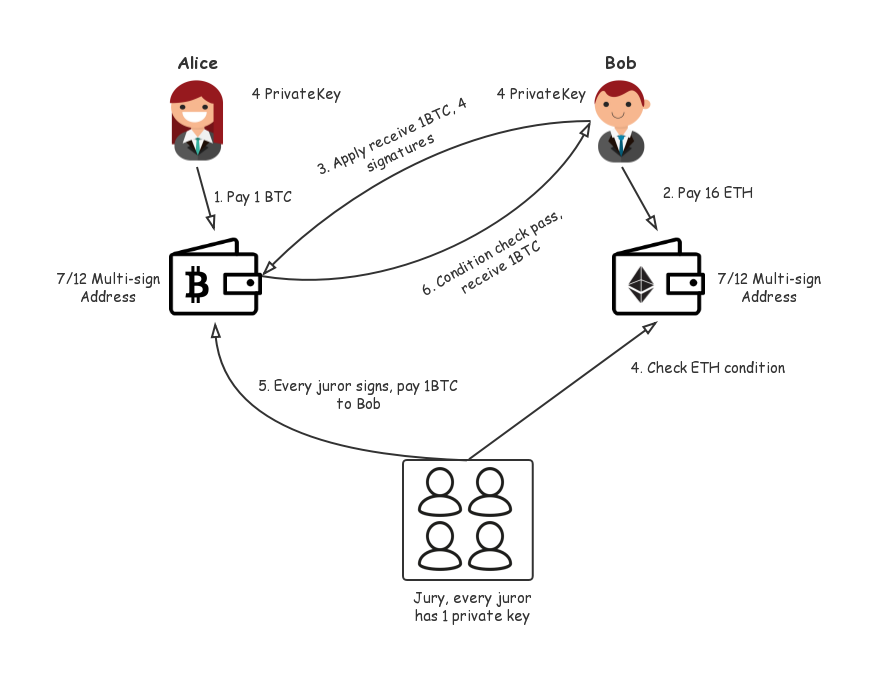
\includegraphics[width=1\textwidth]{./figures/jury.png}
    \centering
    \caption{The normal process of executing the exchange contract (with Jury endorsement)}
    \label{fig:jury}
    \centering
\end{figure}
\begin{enumerate}
    \item Jury members and two user accounts first executed the proper contract that generated 7/12 multi-signature address for both cryptocurrencies.
    \item Then both parties transferred a certain amount of exchange currency to corresponding multi-signature address.
    \item Each party will initiate the signature request with their own four private keys to collect the tokens.
    \item Jury verified the validity of both contracts and checked the status of two multi-signature address. If failed, go back to step 2.
    \item After verifying the satisfaction, each juror will sign with the private key and invoke the transactions.
    \item If one party of this transaction failed or timed-out, the Jury will terminate the contract, and there will be a compensation to the other by the one caused the fault.
\end{enumerate}
\begin{figure}[H]
    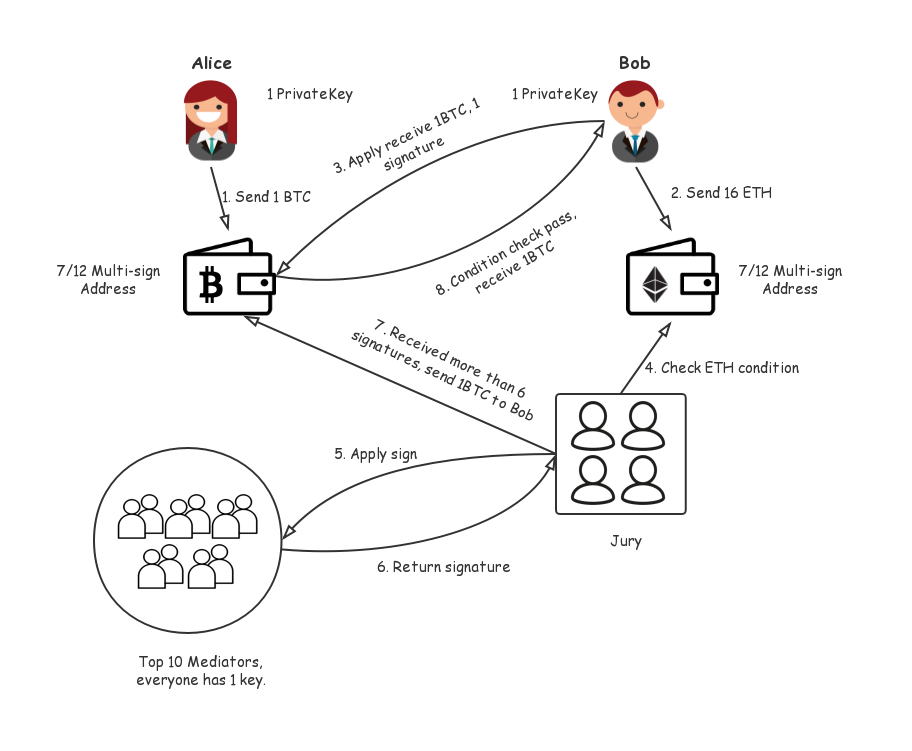
\includegraphics[width=1\textwidth]{./figures/mediator.png}
    \centering
    \caption{The normal process of executing the exchange contract (with Mediator endorsement) }
    \label{fig:mediator}
    \centering
\end{figure}
\noindent The process of Mediator endorsement during the preparation stage differs from the previous one is, the signed contract will inquire the current votes of the Mediator and select the first ten nodes to form the 7/12 multi-signature address. Also, since the limited number of juror in the Jury endorsement, Mediator mode guarantees the persistence of a multi-signature wallet, so there is additional step for the Jury that has already reached the consensus to send the execution results to Mediators to verify, then the jury leader can broadcast the result once received the majority of Mediators' signature.

\noindent Among the projects I have studied so far, PalletOne has the most ambitious and powerful team with a purely technical project that does not have much community operation.